% Compile from this directory with the accompanying figures; run LaTeX twice.
\documentclass[11pt,letterpaper]{article}
\usepackage[margin=1in]{geometry}

\usepackage{booktabs,amsmath,amssymb}
\usepackage{tikz,graphicx,caption}

\captionsetup{font=small,labelfont=bf,hypcap=false}
\captionsetup[table]{position=top,skip=4pt}
\usepackage[hidelinks]{hyperref}
\hypersetup{pdftitle={Sherlock: Replay-Based Identification and Conditional Certification of Minimal Repairs in LLM Agent Workflows},
  pdfauthor={Ali Aan, Ibraheem Farooq, Wajih ur raza}}
\setlength{\parindent}{0pt}
\setlength{\parskip}{5pt plus 1pt}
\setlength{\emergencystretch}{2em}\raggedbottom
\title{Sherlock: Replay-Based Identification and Conditional Certification of Minimal Repairs in LLM Agent Workflows}
\author{\begin{tabular}{@{}ccc@{}}
Ali Aan & Ibraheem Farooq & Wajih ur raza\\
\footnotesize\texttt{i230708@isb.nu.edu.pk} &
\footnotesize\texttt{i230816@isb.nu.edu.pk} &
\footnotesize\texttt{i230819@isb.nu.edu.pk}
\end{tabular}\\[5pt]
\small Department of Computer Science\\
\small National University of Computer and Emerging Sciences Islamabad\\
\small Islamabad, Pakistan}
\date{}
\begin{document}
\maketitle
\begin{abstract}
In an LLM agent workflow, several distinct configuration changes can repair the same failed execution. A successful replay establishes what one change achieves but leaves open whether a maintainer has found every inclusion-minimal repair. Sherlock restores selected node configurations from a passing reference and re-executes the failed workflow from a checkpoint against recorded external replies. We compare two ways to establish coverage when a replay can pass, fail, or leave the intervention unresolved. The production search infers subset failures under monotonicity. A direct-evidence search instead tests candidates in ascending cardinality and omits only sets that already contain a passing witness. On 86 planted failures, production recovered 84 exact families at ten queries and conditionally certified 82. On 40 antagonistic controls it missed every repair, whereas direct search recovered all 40 at a budget of 40, certifying 20. Across all 127 nontrivial three-node predicates with a failed empty set and four inert candidates, production marked 21 incorrect families complete. Direct search certified all 127 at full budget. This assurance has a measurable cost: on 100 monotone workflows, direct search averaged 35.11 queries against 6.67 for forced duality. The choice between these procedures therefore turns on what can be established about the workflow's behavior under additional restores.
\end{abstract}
\section{Introduction}
In a workflow built around a large language model (LLM), a model call can sit between ordinary software components that select evidence, parse a reply, or write the final answer. Each component reads state left by its predecessors. An incorrect answer may first become visible at the last writer even when that writer processed its input correctly. Conversely, a changed intermediate value may be harmless if no successor reads it. Studies of multi-agent traces identify both coordination failures and failures of task verification across systems \cite{cemri,zhang}. For a maintainer who has a reproducible failed check, the immediate question is which changes would make that check pass.

Existing methods offer several ways to narrow the investigation. Who\&When asks which agent made a decisive error and at which step \cite{zhang}. Causal Agent Replay estimates how intervening at a step changes the distribution of later outcomes \cite{shah}. ReplayRCA measures the effect of a proposed replacement action against a paired continuation \cite{replayrca}. A single successful intervention can justify a maintainer's choice to apply that fix. It leaves open whether another change would suffice, whether all parts of a proposed fix are necessary, and what evidence would settle either question.

Consider an invoice for 1,200.50 EUR. A faulty extractor reads the characters before the comma as the entire amount. The normalizer could recover the amount from the raw text, but its current configuration tells it to trust the parsed value. Restoring the extractor repairs the invoice even with the normalizer still configured to trust it. Restoring only the normalizer also repairs the invoice, because the raw text survived the parsing error. A maintainer who cannot change the extractor would have reason to prefer the second repair. Testing the first gives no observation about that option.

We ask for all inclusion-minimal sets of node configurations whose restoration makes a specified check pass on a recorded failure. Each restore takes its configuration from a passing execution of the same task. Minimality means that every proper subset fails. Repairs can have different cardinalities, and two repairs can overlap. Both the reference execution and the set of eligible patches are part of the question. If a restore changes an external request, its response may be absent from the recording. The outcome of that intervention then remains unknown.

This formulation connects two kinds of evidence. Executing a fork supplies a witness for a particular restore. Enumerating minimal subsets supplies an argument about the restores that remain. Delta debugging and constraint reasoning already provide ways to reduce a passing set or exclude regions of a subset lattice \cite{zeller,previti,mcs}. Applying these operations to recorded workflows requires an explicit account of what each query means. In particular, a search that infers failure of a subset from failure of its superset assumes that adding restores can never break a success. Holding external responses fixed does not establish that property.

Sherlock builds candidate patches, reconstructs a checkpoint before the first selected node, and reruns the suffix on recorded replies. Its report distinguishes the sets found from its evidence for completeness. On 86 planted failures, four top-ranked singleton repairs passed replay but omitted an alternative. At ten queries, search recovered the exact family in 84 cases and supported a completeness claim in 82 under its search assumptions. In separate controls where an additional restore could undo the first, the initial feasibility probe missed every repair. We therefore also evaluate a search that uses only direct replay evidence. Its query cost measures the price of certifying the family without assuming that additional restores preserve success.

\begin{itemize}
\item A replay semantics and implementation that connect node-level configuration changes to a fixed task check, including an explicit unknown verdict for unsupported interventions.
\item A direct-evidence certificate for a partial replay oracle, a cardinality-first procedure for obtaining it, and an instance-specific lower bound on the queries required when the oracle is unrestricted.
\item A controlled comparison of repair recovery, certification and query cost under alternative repairs, missing replies, and violations of monotonicity.
\end{itemize}
Section~2 relates these claims to prior work. Sections~3 and~4 describe the method and evaluate its assumptions, respectively. Section~5 concludes.

\section{Related Work}
\paragraph{What can a failed trace establish?}
Who\&When asks a diagnostician to recover an annotated agent and decisive step from a failed multi-agent trajectory. Its results distinguish the two levels of resolution: even the best evaluated method identified the responsible agent more often than it located the decisive step \cite{zhang}. That difference matters when a single agent appears repeatedly in a workflow. A good agent ranking can still leave many possible interventions. MAST approaches trace diagnosis at a different level, using annotated runs across seven frameworks to characterize recurring failure modes \cite{cemri}. Its taxonomy can explain why verification or coordination deserves attention across a population. A category shared by many failures leaves the actionable configurations for any particular run undetermined.

AEGIS starts from successful trajectories, introduces context-sensitive errors, and learns attribution from labeled faulty agents and error modes \cite{aegis}. Its construction makes the injected agent identifiable for evaluation. Who\&When Pro also controls the origin of a fault: it reproduces a successful prefix before introducing the failure and supplies labels across modalities \cite{pro}. This controls an important ambiguity in retrospective annotation. It does not follow that the injected step is the only place a repair can succeed. A downstream component may contain a redundant recovery path, as the invoice normalizer does. Sherlock uses questions and keys from these benchmarks to construct paired executions. Its repair labels come from interventions on those executions. The original public traces support a separate ranking experiment because their labels alone cannot establish which configuration restores pass.

\paragraph{What does replay hold fixed?}
Causal Agent Replay intervenes at an agent step and samples continuations under a stochastic policy. A contrastive estimator locates a pivotal decision, and a Shapley estimator allocates credit across interacting steps. The evaluation uses synthetic causal models with known effects \cite{shah}. This procedure addresses the probability of a successful continuation. A rare success under sampling and a guaranteed success on one recorded reply are different observations. Sherlock fixes the replies and asks a narrower question that can be decided by one supported execution per subset.

ReplayRCA restores the environment preceding a chosen step. It compares continuation after a replacement action with continuation after the original action through the same replay mechanism. Its post-hoc and live-oversight tracks evaluate whether a diagnostician can improve outcomes by intervening once \cite{replayrca}. The placebo controls for variation introduced by continuation, which a simple comparison against the historical failure would confound with the intervention. Finding two disjoint configuration repairs, or a necessary pair whose individual restores fail, requires a different experimental design. It requires a defined universe of configurations and queries about subsets of that universe. A single-action success rate leaves that family unidentified even when estimated precisely.

Li et al. recover inclusion-minimal repair families by replacing messages with their clean counterparts and replaying the workflow \cite{li}. Their Graph-Constrained Joint Replay (GCJR) tests single events and causally incomparable pairs. It recovered the exact family on all 90 in-scope synthetic DAGs and all 24 cases in a model pilot, and abstained on all 30 sequential-joint controls. Sherlock restores node configurations and asks when the observed verdicts certify a family even if some interventions remain unresolved. We did not compare the methods on a common benchmark.

\paragraph{From isolating a change to enumerating alternatives.}
Zeller's work on yesterday's passing version and today's failing version tests subsets of their differences to isolate a failure-inducing change \cite{yesterday}. A passing reference is valuable for the same reason here: it supplies concrete configuration values to try. Zeller and Hildebrandt formalize reduction by repeated tests on subsets and complements and distinguish one-element minimality from stronger notions of minimality. Their testing framework also admits unresolved outcomes \cite{zeller}. A reduction that terminates when no single element can be removed can miss a smaller passing subset when the predicate is non-monotone. Zeller's work on cause-effect chains applies interventions at successive program states to trace how a value difference propagates to a failure \cite{chains}. This motivates recomputing downstream state after a patch. A chain through program states and a family of alternative interventions describe different aspects of the same failure.

Constraint reasoning gives a closer analogue for enumeration. A minimal correction subset identifies constraints whose removal restores satisfiability, with every removal necessary \cite{mcs}. Removing additional constraints preserves satisfiability by construction. Restoring additional agent configurations has no corresponding guarantee. Grégoire, Mazure and Piette exploit the relationship between maximal satisfiable and minimal unsatisfiable sets and use a local-search oracle to accelerate a complete procedure \cite{boost}. Previti and Marques-Silva explicitly study partial enumeration: a method can produce useful minimal unsatisfiable subsets before it exhausts the space \cite{previti}. Sherlock adopts that distinction when it reports a verified repair after a budget expires. Its complement queries use the familiar hitting-set observation that any undiscovered minimal repair must omit at least one member of every known repair. The computational saving arises from the structure of the predicate. The agent-specific difficulty is supplying a verdict whose meaning survives checkpoint restoration and missing responses.

\paragraph{Replay fidelity and the scope of a certificate.}
R2 makes the recording boundary an explicit systems choice. Recording selected interface calls can reduce overhead, provided their results and relevant side effects are reproduced \cite{r2}. The rr system pursues reproducibility at a lower level by controlling sources of nondeterminism in user-space execution \cite{rr}. Both illustrate why replay fidelity depends on which interactions cross the boundary. In Sherlock a request hash identifies the reply to reuse. If a modified request has no recorded reply, executing it live would introduce a different experiment. A matching hash also cannot reconstruct hidden state in a remote service.

Pakhomov and Nijkamp show why repeatability alone is insufficient: two restored copies can agree with each other while diverging from the original continuation if random-stream state was omitted \cite{pakhomov}. Their concern is fidelity of the restored state to the intervention claim. Sherlock additionally needs evidence that the remaining subsets cannot contain another minimal repair. The two requirements are independent. A complete truth table for a misreconstructed fork answers the wrong question, while a faithful replay of one successful restore may leave many alternatives open.

\begin{table}[htbp]\centering\small
\caption{What each study can establish. An unobserved intervention requires an explicit evidential or structural argument before it can support a completeness claim.}
\begin{tabular}{@{}p{.21\linewidth}p{.31\linewidth}p{.41\linewidth}@{}}\toprule
Study & Observation or intervention & Output and coverage condition\\\midrule
Who\&When / Pro & Annotate a trace or inject a labeled fault & Agent or step label. Repair-subset outcomes unmeasured.\\
CAR / ReplayRCA & Replace a decision and sample continuations & Effect estimate or placebo-adjusted success. Alternative configuration sets untested.\\
GCJR & Restore messages and replay & Minimal event sets within a graph-constrained domain of singletons and pairs.\\
Delta debugging & Test subsets of input differences & Reduced example under the test predicate. Unresolved tests constrain minimality.\\
Partial MUS enumeration & Query formula satisfiability & Multiple minimal conflicts. Exhaustion distinguishes partial from complete enumeration.\\
Sherlock & Restore configurations on a recorded fork & Minimal repairs relative to eligible patches. Required verdicts must be observed or entailed under stated assumptions.\\\bottomrule
\end{tabular}\end{table}

Sherlock's contribution is a systems and evaluation result. It gives an operational meaning to a subset query on a recorded LLM workflow and exposes the evidence behind a repair-family claim. Its shrink and complement operations build on established combinatorial methods. The experiments measure how much search these operations save and what happens when the oracle lacks a reply or violates monotonicity.
\section{Materials and Methods}
\subsection{Datasets and workflow corpus}
Table~\ref{tab:corpus} distinguishes a workflow definition, an execution of that workflow, and a query about one execution. Reordering the candidates or changing the budget preserves the underlying execution. The runtime corpus pairs solver runs around one recorded model reply per question. The planted teams use a deterministic stub where a model is needed. The public traces have attribution labels but lack the paired state and replies required for repair evaluation.

\begin{table}[htbp]\small\centering
\caption{Units of evaluation and repair structures. Joint denotes a repair requiring multiple nodes. Alternatives are distinct inclusion-minimal sets for one failure.}\label{tab:corpus}
\begin{tabular}{@{}p{.16\linewidth}p{.31\linewidth}p{.46\linewidth}@{}}\toprule
Group & Base units and derived cases & Eligible patches and target families\\\midrule
Planted teams & 7 graphs, 52 visible and 34 seeded hidden failures, 3 harmless controls & 41/44/1 failures with 1/2/3 candidates. Gold has one singleton (52), one pair (29), one triple (1), or two singletons (4).\\
Runtime solver & 1 graph, 7 nodes, 185 retained questions, 6 conditions each & 740 singleton and 370 joint-pair conditions. A decoy adds one candidate in half the conditions.\\
Search oracles & 100 generated test workflows, 11 candidate orders each & 1--8 candidates. Exhaustive tables give one minimal repair each: 41 singletons and 59 pairs.\\
Controlled circuits & 4 monotone templates $\times$ 4 sizes $\times$ 10 assignments, plus 40 antagonistic controls & 80 singleton or joint controls and 80 two-pair cases. Withholding a verdict reuses the same circuit.\\
Selector check & 80 further assignments on the same 4 monotone templates & 4 or 8 candidates, 10 fresh seeds per size and template.\\
Public ranking & 5,032 labeled traces, 4,112 included & 2,364 AEGIS and 1,748 Who\&When included. Excluded 920 two-role MathChat traces. Repair families unobserved.\\\bottomrule
\end{tabular}\end{table}

The planted teams span vendor briefs, order handling, invoices, support and finance, including graphs with 32--33 nodes. The harness removes subsets of planted faults and executes the check to construct gold independently of the search order. Harmless writes and designed tape misses are retained. Hidden cases use new seeded combinations of the same teams and fault catalogs.

The runtime corpus takes questions and short answer keys from the pinned datasets \href{https://huggingface.co/datasets/Fancylalala/AEGIS/tree/b936269a5143e4450242d8628bff026bdc5bae18}{Fancylalala/AEGIS} and \href{https://huggingface.co/datasets/Leoxx/whowhen_pro/tree/0bd196c8a040841c4ae167ab33cc8151de246f1f}{Leoxx/whowhen\_pro} \cite{aegis,pro}. Eligibility required a text-only task, a unique question and a nonempty normalized key of at most 32 characters absent from the question. The first 50 eligible questions in each of six benchmark strata were pooled and shuffled with seed 20261117. The seven-node graph reads the question, applies bias, preface and steering stages, calls the model once, then extracts and formats its answer. Each question supplies one recorded reply shared by clean and failed runs.

Of 300 attempts, 115 failed normalized exact match on the clean run, including incorrect answers and precision or formatting differences. The six strata retained 50, 44 and 30 of 50 for AEGIS GSM8K, MATH and SciBench, and 36, 21 and 4 of 50 for Who\&When Pro math, scibench and simpleqa\_verified. Subsequent checks required absence of the key from the request, identical solve writes, failure of the planted run, exhaustive agreement with the assigned repair, failure of its proper subsets, exclusion of the decoy, supported offline calls and agreement of production diagnosis with gold. The generation report records zero additional exclusions or rule failures. The released question-level replay export contains the 185 retained recordings. A reviewer read all 30 pilot transcripts before use of the corpus. Collection of the full run began before that review. Each retained question was later crossed with three fault assignments (truncate at extraction, add a prefix at formatting, or both) and an unused-field write on or off. Five of the six assignments per question played no role in retention.

For the generated test split, the experiment executes every eligible subset to construct a Boolean verdict table before comparing search policies. The separate controlled circuits pass an answer through restored stages on one or two branches. A broken stage drops the answer. The four monotone templates contain one singleton, one joint pair, two disjoint pairs, or two pairs sharing a stage. The original circuits cross sizes 5, 6, 7 and 9 with ten assignments each. The antagonistic template adds a stage whose restoration suppresses the otherwise correct answer. Gold is computed by comparing every passing subset with all its proper subsets.

\subsection{Architecture and intervention semantics}
\begin{figure}[htbp]\centering
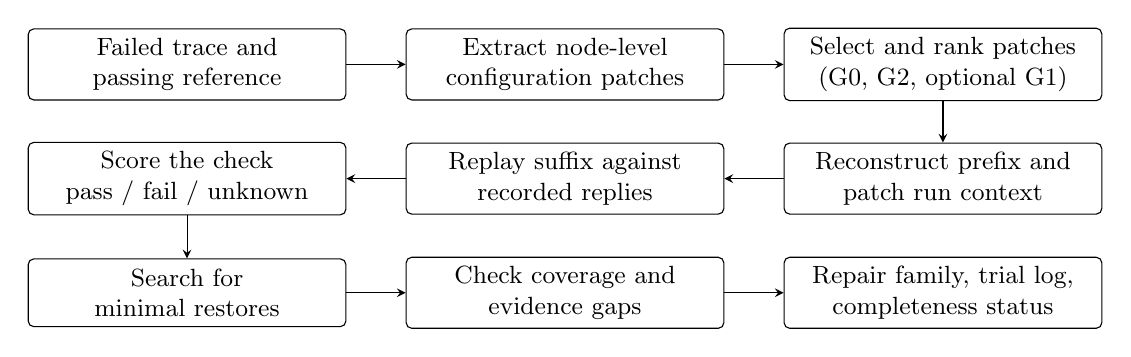
\begin{tikzpicture}[every node/.style={draw,rounded corners=2pt,align=center,text width=3.8cm,minimum height=.86cm,font=\small},>=stealth]
\node (a) at (0,0) {Failed trace and\\passing reference};
\node (b) at (4.8,0) {Extract node-level\\configuration patches};
\node (c) at (9.6,0) {Select and rank patches\\(G0, G2, optional G1)};
\node (d) at (9.6,-1.45) {Reconstruct prefix and\\patch run context};
\node (e) at (4.8,-1.45) {Replay suffix against\\recorded replies};
\node (f) at (0,-1.45) {Score the check\\pass / fail / unknown};
\node (g) at (0,-2.9) {Search for\\minimal restores};
\node (h) at (4.8,-2.9) {Check coverage and\\evidence gaps};
\node (i) at (9.6,-2.9) {Repair family, trial log,\\completeness status};
\foreach \x/\y in {a/b,b/c,c/d,d/e,e/f,f/g,g/h,h/i}{\draw[->] (\x)--(\y);}
\end{tikzpicture}
\caption{One trial reconstructs and executes a fork. Search requests further subsets through the same replay operation until coverage or a stopping condition is reached.}
\end{figure}

\begin{figure}[htbp]\centering
$\boxed{\text{extract }(E)}\longrightarrow\boxed{\text{normalize }(N)}
\longrightarrow\boxed{\text{validate}}\longrightarrow\boxed{\text{post}}$\\[4pt]
\small
\begin{tabular}{@{}llrr@{}}\toprule
Restore & Normalizer action & Amount (EUR) & Posted (USD)\\\midrule
Neither (failed run) & Use parsed amount & 1.00 & 1.10\\
$E$ alone & Use parsed amount & 1,200.50 & 1,320.55\\
$N$ alone & Reparse raw text & 1,200.50 & 1,320.55\\
Both (reference) & Reparse raw text & 1,200.50 & 1,320.55\\\bottomrule
\end{tabular}
\caption{The invoice example. Restoring either configuration suffices because the normalizer receives both the parsed amount and the raw text. Validation and posting rerun on the resulting state.}\label{fig:invoice}
\end{figure}

In Figure~\ref{fig:invoice} the eligible set is $C=\{E,N\}$. More generally, $C$ contains executed nodes retained by the eligibility rules for which the passing run supplies a context patch. For $S\subseteq C$, a fork applies precisely those patches in the failed context. Let $b(S)$ denote the Boolean task check on the stipulated execution when defined, and let $v(S)\in\{\mathrm{pass},\mathrm{fail},\mathrm{unknown}\}$ denote the observation available on tape. An unknown supplies no Boolean constraint. For a total Boolean behavior with passing family $P=\{S:b(S)=1\}$ the target is
\[
\mathcal M(b)=\{S\in P:\ \not\exists\, T\in P\text{ with }T\subseteq S,\ T\ne S\}.
\]
A passing witness establishes sufficiency. Evidence for minimality must also exclude every passing proper subset. Evidence for a complete family must exclude every other minimal repair. Formally, every total behavior consistent with the evidence and the declared assumptions must yield the reported family. This criterion presupposes faithful replay, fixed patch semantics, a fixed check and an explicit candidate universe. Extending the claim to additional nodes would require justifying their exclusion.

\begin{center}\begin{minipage}{\linewidth}\centering
\captionof{table}{All three joint restores pass. The singleton evidence determines which reports the observations support.}\label{tab:audit}
\small\begin{tabular}{lrrrr}
\toprule
Repair pattern & Neither & First & Second & Both \\
\midrule
Alternative singletons & Fail & Pass & Pass & Pass \\
Joint repair & Fail & Fail & Fail & Pass \\
Missing singleton replies & Fail & Unknown & Unknown & Pass \\
\bottomrule\end{tabular}
\end{minipage}\end{center}

The last row admits a Boolean completion in which the pair is necessary and another in which a singleton passes. Both agree with the observed requests, even if monotonicity is assumed. More search on the same four cells cannot resolve the ambiguity. An unknown elsewhere can be harmless if all admissible completions have the same minimal family.

\subsection{Candidate identification and replay execution}
G0 ranks clues such as execution errors and changed writes. G2 excludes nodes after the last writer of the checked field, nonwriters parallel to that writer, unchanged writes unless a widening clue applies, and context restores that have no effect. A missing known-good configuration is recorded as untestable. Equality of writes on the original run is a filter, not an invariance proof for all counterfactual inputs. G1 optionally scores node evidence cards to break ties among G0 clues. G3 performs the intervention. The record associates run and thread identifiers, checkpoint history and per-node writes with run contexts and recorded request/reply pairs.

\begin{center}\begin{minipage}{.96\linewidth}\hrule\smallskip
\textbf{Algorithm 1. Candidate construction and replay verdict}\\
\textit{Inputs} Failed and passing traces, tape, selected nodes $S$, task check.\\
\textit{Outputs} Eligible order, verdict, fork evidence or reason for abstention.
\begin{enumerate}\setlength{\itemsep}{0pt}
\item Compare contexts and assign changed entries to named nodes. Record untestable nodes, apply G2, then order eligible patches by G0 and optional G1.
\item If the reference or required patch is unavailable, return unknown for the requested intervention. For the empty subset, use the original check.
\item Locate the earliest restored node. Reconstruct its prefix in a fresh LangGraph thread from recorded writes and locate the fork checkpoint.
\item Apply the selected context patches and resume the workflow. Recompute downstream writes from the resulting state.
\item Match each intercepted external request to its recorded reply. On a miss or an invalid fork, stop and return unknown with the reason.
\item Validate prefix and restore evidence. Evaluate the fixed check on the recomputed output and return its verdict with the trial record.
\end{enumerate}\hrule\end{minipage}\end{center}

The server experiment uses \href{https://docs.langchain.com/oss/python/langgraph/use-time-travel}{LangGraph checkpoint histories} and superstep forks through its in-memory runtime. Each recording has an isolated SQLite copy. Model requests use exact-hash replay and external sockets are blocked. Sampling occurs during original recording only. The guarantee requires that state influencing the check be reconstructed or held fixed. Mutable remote state, unrecorded side effects and uncontrolled nondeterminism fall outside that condition.

\subsection{Minimal repair search and conditional certification}
For a total Boolean oracle, monotonicity means $b(S)=1\Rightarrow b(T)=1$ whenever $S\subseteq T\subseteq C$. Under this assumption a failing superset excludes all its subsets. Failure of each immediate child of a passing set then implies failure of every proper subset. Monotonicity can be checked on a complete finite verdict table by inspecting every adjacent pair or established from the semantics of a circuit. Repeated execution of the same queries cannot establish it on an arbitrary new workflow. Production search assumes this property and has no automatic detector.

\begin{center}\begin{minipage}{.96\linewidth}\hrule\smallskip
\textbf{Algorithm 2. Bounded search and interpretation of its report}\\
\textit{Inputs} Ordered $C$, oracle $v$, trial, time and size limits, assumptions for interpreting coverage.\\
\textit{Outputs} Repair candidates, unverified passes, evidence log and completeness status.
\begin{enumerate}\setlength{\itemsep}{0pt}
\item Cache each queried subset. Before a new trial, check the time and query limits. On exhaustion, return the accumulated report as incomplete.
\item For $|C|>1$, probe $C$. On failure, production stops with no repair and an incomplete status. An unknown cannot exclude the subsets.
\item If $|C|>6$ and at least $|C|+2$ trials were budgeted, query complements formed by omitting one node from every repair found so far. Initially the complement is $C$.
\item Shrink a passing complement by deleting low-priority chunks, halving the chunk size down to one. Retain a deletion only on a pass. Record the result, marking a pass unverified if a queried proper subset is unknown. Continue complement search with the enlarged family.
\item If every complement fails, coverage follows under monotonicity. On unresolved coverage or more than 64 combinations, use enumeration. Small lists enter enumeration directly.
\item Enumerate by highest candidate index, then size up to the size limit. Skip supersets of recorded passing sets. Log verdicts and record new passes as in step 4.
\item Return the family and log. Production sets its flag on a nonempty verified family only with coverage, no exhaustion, no untestable nodes and no queried unknowns. Interpret a flag that relies on monotone pruning as conditional on that assumption.
\end{enumerate}\hrule\end{minipage}\end{center}

Every undiscovered minimal repair omits at least one element of every known passing set. It must therefore fit inside at least one complement tested in step~3. Under monotonicity a failure at each such complement rules out every remaining repair. Without monotonicity the initial full-set probe alone can discard the only passing singleton, as the antagonistic controls demonstrate. Where monotonicity is unestablished, a reader can still verify a directly observed pass and inspect its tested proper subsets. A claim based on inferred failures remains conditional. The exhaustive baseline can establish a family on a fully observed table without monotonicity. It is a separate comparator. The deployed selector does not automatically switch policies when monotonicity fails.
\paragraph{A certificate without monotonicity.}
Consider any proposed family $F$ of pairwise incomparable subsets. With an otherwise unrestricted Boolean oracle, the following two conditions are necessary and sufficient for the observations to certify $F$. First, every member of $F$ has an observed pass. Second, every subset containing no member of $F$ has an observed failure. The initial failed execution supplies the empty-set observation.

For sufficiency, the second condition makes every proper subset of a member of $F$ fail. Any remaining set contains a member of $F$ and hence cannot be a new minimal repair, whatever its verdict. For necessity, an unwitnessed member can be assigned failure in a compatible completion. Likewise, an undecided set containing no member of $F$ can be assigned success. Some minimal passing subset of that set must then lie outside $F$. Each missing observation can thus change the answer. On a fully observable instance, these two conditions give a lower bound of one query per member of $F$ and one per nonempty set containing no member of $F$.

We implement this criterion in the evaluation as \emph{direct search}. Visit nonempty sets by increasing cardinality and skip any set containing an already observed pass. A new passing set is confirmed minimal if none of its proper subsets remains unresolved. Even an unconfirmed pass can exclude its strict supersets from minimality. A queried unknown that contains no earlier pass leaves coverage open, as does hitting the budget with an uncovered set still to test. With full Boolean evidence this order queries exactly the sets in the lower bound. The bound concerns a complete certificate in a black-box model. Earlier discovery of one repair and lower elapsed runtime are different objectives. On fully known tables this procedure is the existing ascending-pruned baseline; the extension specifies its partial-evidence semantics and checks its certificate without monotone inference.

\section{Experimental Results and Analysis}
\subsection{Experimental setup}
\begin{table}[htbp]\centering\small
\caption{Recording and evaluation configurations. The recording model and the optional ranking model serve different purposes.}
\begin{tabular}{@{}p{.24\linewidth}p{.69\linewidth}@{}}\toprule
Component & Configuration\\\midrule
Solver recording & llama.cpp server build \texttt{b1-161755f29}, Ollama tag \texttt{qwen3.8:27b-mtp-q8\_0}, GGUF Q8\_0. Two NVIDIA RTX PRO 4000 Blackwell GPUs, 24 GB each.\\
Model call & Short-answer prompt ending in \texttt{\#\#\#\# <answer>}, no units. Request effort \texttt{xhigh}, 120,000-token cap, temperature 1.0, top-$k$ 20, top-$p$ 0.95, min-$p$ 0.05, random sampling seed. Model and template hashes in \texttt{data/sherlock-replay-corpus/model.json}.\\
Server replay & Debian 13, Xeon 3.10 GHz, 8 cores/16 threads, about 63 GiB RAM. Python 3.13.5, LangGraph 1.2.15, API 0.16.0, in-memory runtime 0.36.0, HTTPX 0.28.1, SQLite 3.46.1. Local ASGI TestClient, 48 isolated workers per pass.\\
Search & Planted caps 3, 10, 40, enumeration limit 3. Server caps 1--7 and 40. Generated caps 3, 10, 40 and full ($2^{|C|}-1$), all sizes unless stated. Default time budget 10 minutes.\\
Ordering & Gemini 2.5 Flash for archived hosted scoring. Search permutations and original circuit assignments use seeds 0--9. Bootstrap seed 185.\\\bottomrule
\end{tabular}\end{table}

The \href{https://github.com/aliaankhowaja/sherlock-research}{Sherlock repository} includes the locked environments, corpus manifests, raw trials and scoring scripts. From its root, \texttt{bash scripts/final-ablations.sh /tmp/sherlock-new} regenerates the paired ablations in a fresh directory. Archived repeats agree on 89 planted records and 29,200 search rows. Server results under \path{docs/eval/replay_corpus/final/langgraph/} use separate processes and fresh cassette copies on each pass. The earlier linear adapter and the repeated server pass operate on the same recordings.

\subsection{Evaluation metrics and protocols}
For a reported family $\widehat{\mathcal M}$ and gold family $\mathcal M$, exact recovery is the indicator of $\widehat{\mathcal M}=\mathcal M$. Every nonempty report unequal to gold counts as wrong, including one that contains only valid repairs but omits an alternative. An empty report on a failure counts as abstention. Certified-and-exact recovery requires exact recovery and a supported completeness flag under the stated protocol. A method can match gold before enough evidence has accumulated to distinguish it from another possible family. A query is a distinct restore subset requested by one method on one diagnosis. Reusing its cached verdict within that diagnosis adds no query. Search-oracle queries are logical accesses to verdict tables. Server forks are actual checkpoint executions.

The primary ablations pair the same planted case or generated workflow across policies. The protocol fixed three contrasts locally after earlier benchmark results were available and before running the ablations. Percentile intervals use 10,000 paired bootstrap draws. For planted cases we resample cases within each fixed team, preserving team sizes. For generated workflows we first average the archived order and ten permutations within each workflow, then resample workflows. Two-sided sign tests omit ties, with Holm adjustment over the three contrasts. Runtime comparisons average six paired conditions within each question and resample whole questions. Exact McNemar tests use the binary endpoint of all six conditions correct per question, with Holm adjustment across three baseline comparisons. These analyses condition on the teams and fault structures represented.

For public traces, mean reciprocal rank (MRR) averages the reciprocal rank of the first labeled agent. Trials to label counts subset proposals in the ordered search until the labeled set is reached. Both metrics use published labels. Neither requires a replay oracle. Hosted ranking on planted cases instead measures actual recovery and logical forks, averaging five passes within each eligible case.

\subsection{Results and analysis}
\begin{center}\begin{minipage}{\linewidth}\centering
\captionof{table}{Primary ablation results. Endpoints, in order, are wrong collections prevented, gain in complete exact recovery at ten forks, and queries saved over priority enumeration. W/T/L counts paired improvements, ties and regressions.}\label{tab:primary}
\small\begin{tabular}{lrrr}
\toprule
Paired intervention & Mean effect & 95\% interval & W/T/L \\
\midrule
Verify proposed singleton & 38.37 pp & [29.07, 47.67] & 33/53/0 \\
Enable candidate pruning & 0.00 pp & [0.00, 0.00] & 0/86/0 \\
Force duality search & 29.35 queries & [21.54, 38.18] & 91/9/0 \\
\bottomrule\end{tabular}
\end{minipage}\end{center}

\textbf{Does verification improve the proposal?} Removing only the requirement for a passing fork isolates how often a persuasive proposal fails its own intervention test. Its benefit was converting a wrong claim into an abstention. Testing the same node preserved all 49 exact collections and removed 33 wrong claims (Table~\ref{tab:verify}). All 30 cases requiring a joint repair changed from wrong singleton claims to abstentions. Among the other 56 cases, four verified singletons remained incomplete diagnoses: each had a second valid singleton. Searching for alternatives recovered all four. The wrong-claim reduction persisted when each team was omitted in turn (34.3--44.1 percentage points).

\begin{center}\begin{minipage}{\linewidth}\centering
\captionof{table}{Verification and search ablation. Every row uses the same 86 failed runs and known-good sources. Joint exact counts recovery on the subset requiring at least two nodes in a repair.}\label{tab:verify}
\small\begin{tabular}{lrrrr}
\toprule
Allowed operation & Exact & Wrong & Abstain & Joint exact \\
\midrule
Propose top singleton & 49 & 37 & 0 & 0/30 \\
Verify that singleton & 49 & 4 & 33 & 0/30 \\
Search eligible sets (cap 10) & 84 & 0 & 2 & 28/30 \\
\bottomrule\end{tabular}
\end{minipage}\end{center}

\textbf{Does ranking or pruning change the outcome?} We switched G0 priority and G2 filtering independently, leaving replay active. Each configuration retained the gold nodes in all 86 cases. At cap 10, G2 saved two queries on each of seven cases and zero on the other 79. The zero paired recovery effect in Table~\ref{tab:primary} is an observed tie for every case. With G2 enabled, 41 cases had one eligible candidate, 44 had two, and one had three. At cap 10 production queried every nonempty subset on all 86 cases. None reached the duality threshold of seven candidates. G0 had no aggregate effect on these endpoints. Lowering the cap from ten to three reduced exact recovery to 83 and certified recovery to 81 in every configuration. The three-node support-desk example below accounts for this difference.

\begin{center}\begin{minipage}{\linewidth}\centering
\captionof{table}{Factorial gate ablation on 86 failures. Recovery columns and the first query column use cap 10. The final column gives total queries at cap 3. Each method receives the same patches that change the failed context before filtering.}\label{tab:gates}
\small\begin{tabular}{llrrrr}
\toprule
G0 order & G2 filter & Exact & Certified & Queries (10) & Queries (3) \\
\midrule
On & On & 84/86 & 82/86 & 180 & 176 \\
Off & On & 84/86 & 82/86 & 180 & 176 \\
On & Off & 84/86 & 82/86 & 194 & 190 \\
Off & Off & 84/86 & 82/86 & 194 & 190 \\
\bottomrule\end{tabular}
\end{minipage}\end{center}

\textbf{When does production withhold its completeness flag?} Two cases account for the gap between 84 exact families and 82 completeness flags at cap 10. In the support-desk case with the stale customer profile and the SLA typo, restoring customer lookup alone passed and restoring the standard SLA alone failed. In the revenue case with the 1,000 USD outlier cutoff and the incorrect warning text, restoring the outlier filter alone passed and restoring the quality note alone failed. Both joint trials returned an unknown verdict. The archived trials record no reason for either joint verdict. In each case the two singleton verdicts already determine the family because the pair contains a passing singleton. Production nevertheless withholds its flag after any queried unknown. Two separate planted cases ended with an \texttt{unrecorded\_call} abstention. Three harmless controls were recognized as already passing.


\paragraph{Runtime experiment: crossing faults with a decoy}\label{sec:runtime}
For each of 185 retained questions we toggled a write to an unused field under each of three fault assignments. Every method saw the same failed and passing runs. Naming every changed write introduces a false positive whenever it includes the decoy; restricting replay to singletons cannot recover a required pair. Table~\ref{tab:runtime} measures the two failure modes separately.

\begin{center}\begin{minipage}{\linewidth}\centering
\captionof{table}{Runtime baselines across 1,110 interventions. Each question contributes six paired measurements on the same solver.}\label{tab:runtime}
\small\begin{tabular}{lrrrr}
\toprule
Method & Exact & Wrong & No set & Mean forks \\
\midrule
Sherlock & 1110 & 0 & 0 & 3.00 \\
All changed writes & 370 & 740 & 0 & 0.00 \\
Singleton restores & 740 & 0 & 370 & 1.83 \\
Exhaustive restores & 1110 & 0 & 0 & 3.00 \\
\bottomrule\end{tabular}
\end{minipage}\end{center}

Of the 740 incorrect diagnoses from all changed writes, 555 included the decoy. The other 185 occurred with the extraction fault alone and the decoy off. The faulty extractor changed the formatter's input, so the baseline named both nodes even though restoring extraction alone repaired the output. Testing singletons eliminated wrong nonempty claims, but returned no set on every joint fault. At cap 40 Sherlock certified all 1,110 exact families. Exhaustive replay recovered the same families at the same mean cost. This graph supplies no observed efficiency advantage for Sherlock over exhaustive replay. With one causal fault and no decoy Sherlock needed one fork. With either a second fault or a decoy it needed three. The combination required seven on every question.

\begin{center}\begin{minipage}{\linewidth}\centering
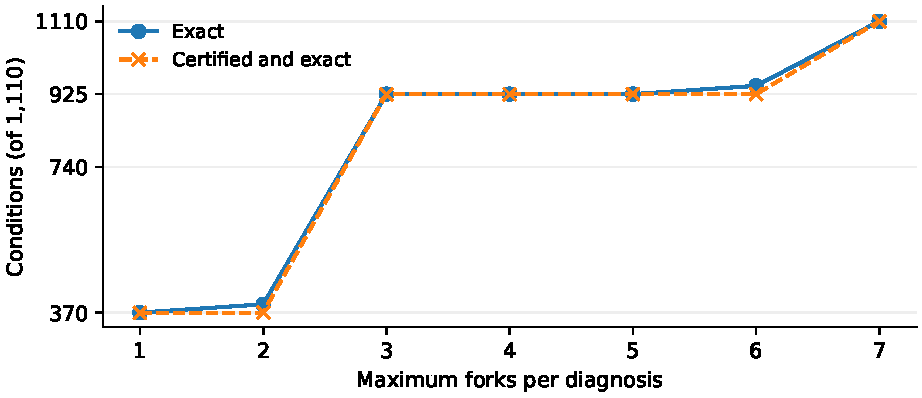
\includegraphics[width=.92\linewidth]{figures/budget.pdf}
\captionof{figure}{Query budget intervention. At cap 6, 946 collections matched gold, but only 925 had a completeness certificate. The last query closed the hardest cell.}\label{fig:budget}
\end{minipage}\end{center}

Separating the assignments used in retention gives 185/185 exact original assignments and 925/925 exact additional assignments at cap 40. Only the original assignment was subject to the diagnosis-agreement gate.  The invariant gains over weaker baselines reflect the fault templates shared by every question. Two independent executions matched trial orders, verdicts and sets, including a separate request-changing control. There the joint restore passed while both singleton requests missed the tape.


\paragraph{Search ablation: what drives the query savings?}\label{sec:search}
We held the verdict table and candidate order fixed and forced each search branch on the same workflow. The production selector switches above six candidates when the query budget allows. Figure~\ref{fig:size} shows why its aggregate mean obscures an important cost: going from six to seven candidates changes both workload size and the algorithm used. Forcing a branch lets us compare strategies at each size.

\begin{center}\begin{minipage}{\linewidth}\centering
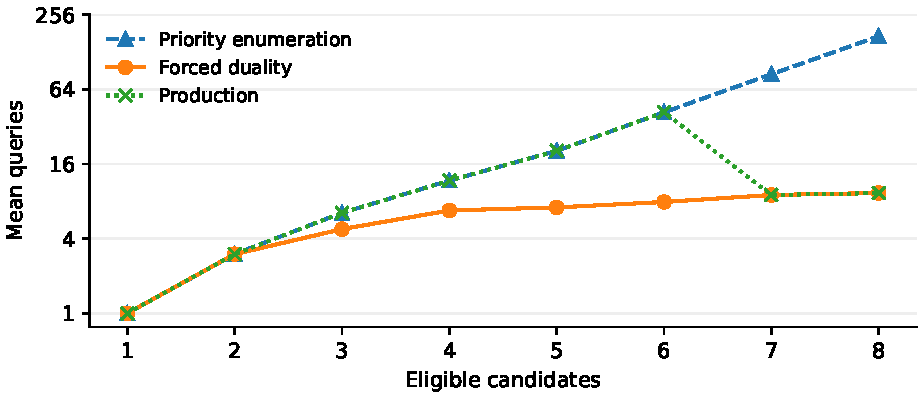
\includegraphics[width=.92\linewidth]{figures/size.pdf}
\captionof{figure}{Full-range search on the archived order. Points average 2, 7, 22, 16, 14, 20, 13 and 6 workflows at candidate counts 1 through 8. The vertical scale is logarithmic. Coincident curves indicate the selector used that branch.}\label{fig:size}
\end{minipage}\end{center}

\begin{center}\begin{minipage}{\linewidth}\centering
\captionof{table}{Search-strategy ablation. Means count distinct queries to completion on the original order. The last column uses actual capped runs with all subset sizes allowed.}\label{tab:cost}
\small\begin{tabular}{lrrrr}
\toprule
Search policy & All 100 & 1--6 (81) & 7--8 (19) & Certified by 40 \\
\midrule
Exhaustive & 52.92 & 26.06 & 167.42 & 61/100 \\
Ascending, prune supersets & 35.11 & 17.27 & 111.16 & 70/100 \\
Forced priority enumeration & 36.06 & 18.21 & 112.16 & 70/100 \\
Forced duality & 6.67 & 6.10 & 9.11 & 100/100 \\
Production & 16.48 & 18.21 & 9.11 & 89/100 \\
\bottomrule\end{tabular}
\end{minipage}\end{center}

On the archived order at full range, production used 1,648 queries versus 3,511 for ascending search, a 53.1\% reduction. Yet production lost on 76 of the 81 smaller workflows and tied on five. It won on every larger workflow. Relative to ascending search, its paired mean savings were 18.63 queries (95\% interval 10.56--27.88).

Averaging eleven orders within each workflow, forced duality saved 12.09 queries below the switch (95\% interval 9.23--15.21) and 102.90 above it (83.36--123.69) over forced enumeration. The primary effect was positive on 91 workflows and zero on nine. Holm-adjusted sign-test $p$-values for verification, pruning and search were $4.66\times10^{-10}$, $1$, and $2.42\times10^{-27}$, respectively. These tests concern the direction of paired differences; the intervals in Table~\ref{tab:primary} concern their mean. With its additional default size limit of three, production certified only 50/100. The threshold of six is the archived production setting. The original comparison provides no evidence that it is optimal.

\textbf{Does removing the size threshold transfer to new circuit assignments?} After examining the archived comparison, we fixed a rule that attempts duality at every size whenever the existing budget guard permits it. We evaluated it against production on 80 further circuit assignments, crossing four monotone templates with sizes 4 and 8 and fresh seeds 10--19. Both policies received the same natural node order and complete oracle. At full range the revised rule used 893 queries (11.16 per assignment) and production used 1,008 (12.60). Both certified all 80 exact families. The 40-query cap gave the same counts. Assignment-level results are in \path{docs/eval/final_ablations/selector_holdout.csv}. At size eight the policies select the same branch, so the saving comes entirely from size four. This post-hoc test holds out assignments and size/seed combinations, while retaining the original circuit mechanisms.


\paragraph{Evidence ablations: alternatives, missing replies and antagonism}\label{sec:evidence}
One successful restore cannot show that a different repair is unavailable. We constructed 80 circuits with two alternatives and 80 singleton or joint-pair controls. Holding node assignments fixed, we first capped search at 40 queries, then separately removed a verdict from the full-range oracle. For singleton templates the missing query was the repair itself; for pair templates it was one singleton child of the first pair.

\begin{center}\begin{minipage}{\linewidth}\centering
\captionof{table}{Controlled circuit ablations. Each cell gives exact / certified-and-exact counts out of 40. Full evidence and one withheld verdict use full-range budgets. Mean queries use full evidence and full range.}\label{tab:evidence}
\small\begin{tabular}{lrrrr}
\toprule
Repair structure & Full evidence & Cap 40 & One withheld & Mean queries \\
\midrule
One singleton & 40/40 & 40/40 & 0/0 & 16.23 \\
One joint pair & 40/40 & 40/30 & 14/14 & 24.15 \\
Two disjoint pairs & 40/40 & 40/40 & 14/14 & 24.73 \\
Two overlapping pairs & 40/40 & 40/30 & 14/14 & 26.20 \\
\bottomrule\end{tabular}
\end{minipage}\end{center}

All 80 alternative-repair cases were complete and exact at full range. At cap 40 all 80 alternative families matched gold. Search certified all 40 disjoint families and 30 of the 40 overlapping families. Withholding the passing singleton eliminated its only direct witness in all 40 singleton cases. Withholding a child of a pair had a different effect: 14/40 cases in each pair template could still be certified. A larger observed failure can rule out the missing child under monotonicity. Production withholds its flag on a queried miss. A withheld cell can still be settled indirectly when the search never queries it. All 42 successful withheld-verdict certificates occurred at sizes seven and nine. The audit checked each returned repair against the verdicts available to that method and found no unsupported claims.

\paragraph{What does certification without monotonicity cost?}
We conducted a post-hoc paired comparison on the archived server verdict tables, the antagonistic controls and the generated monotone workflows. Policies receive the same oracle within a case. A new finite census tests interactions beyond the antagonistic template. Enumerate all $2^7-1=127$ nonempty choices of passing inputs among the seven nonempty subsets of three active nodes. Keep the empty input failing and append four inert candidates to every instance. This fixes the search order (active nodes first) and exercises the production duality branch at seven candidates. The census exhausts this specified function class. Frequencies over it describe algorithm behavior under equal weighting of predicates, not the prevalence of these interactions in deployed workflows.

\begin{center}\begin{minipage}{\linewidth}\centering
\captionof{table}{Paired query-policy results. Each policy cell reports exact families, exact families flagged complete, and mean queries, in that order. A flag from production carries its monotonicity assumption. Full permits all nonempty subsets. Runtime entries use archived server verdicts.}\label{tab:direct}
\small\begin{tabular}{@{}llrr@{}}\toprule
Cases & Cap & Production & Direct search\\\midrule
Runtime conditions (1,110) & 40 & 1,110 / 1,110 / 3.00 & 1,110 / 1,110 / 2.50\\
Antagonistic controls (40) & 40 & 0 / 0 / 1.00 & 40 / 20 / 32.00\\
Antagonistic controls (40) & Full & 0 / 0 / 1.00 & 40 / 40 / 92.00\\
Three-node census (127) & 40 & 43 / 43 / 4.86 & 127 / 64 / 34.58\\
Three-node census (127) & Full & 43 / 43 / 4.86 & 127 / 127 / 46.38\\
Monotone workflows (100) & Full & 100 / 100 / 16.48 & 100 / 100 / 35.11\\\bottomrule
\end{tabular}\end{minipage}\end{center}

Table~\ref{tab:direct} distinguishes finding the right answer from knowing when to stop. At 40 queries, direct search found every census family but could establish coverage for only 64. Production issued 64 completeness flags at either budget, of which 21 accompanied an incorrect family. One predicate makes the error inspectable. Call the active nodes $a,b,c$. The check passes precisely when the active restore is $\{b\}$ or $\{a,b,c\}$. Starting from full restoration, production shrank to the triple. All three pairs failed, so removing one node at a time could make no progress. Its complement probes also failed. It reported the triple as the complete family after eleven queries without testing $\{b\}$, the only minimal repair. The same failure persists across candidate orders. Repeating the full census at each of the 35 choices of active positions among seven candidates yielded 64 production flags per placement, with 21--34 incorrect flags. These are repeated measurements on the same 127 predicates. A passing full restore is therefore insufficient evidence to select the monotone branch.

On the runtime matrix, direct search used 2,775 logical queries against 3,330 production forks, a saving of 555 (16.7\%) at equal certified recovery. Each question contributes the same saving of three queries across its six conditions. Each of the three decoy-on conditions saves one query on a strict superset of the repair. These costs were computed by querying archived results of actual forks; the comparison measures no new server latency. In the separate request-changing control, both policies observed the joint pass and two missing singleton replies and certified no repair. As an independent implementation check we compared direct search with all compatible Boolean completions of each of the $3^7=2{,}187$ three-valued tables over three candidates and a failed empty set. In every table its confirmed sets equaled the intersection of the possible minimal families, and its completeness flag agreed with whether those families were identical.

The larger monotone workflows show the opposite cost ordering. At full range direct search used 3,511 queries, forced duality 667, and exhaustive enumeration 5,292. On the antagonistic controls the corresponding totals were 3,680, 40, and 7,320; forced duality's 40 queries produced only abstentions. Savings from monotone inference have a clear interpretation only when its premise is justified independently. The executable comparison and case-level outcomes are in \path{python/sherlock/eval/evidence_search.py} and \path{docs/eval/final_ablations/evidence_search.csv}.

\textbf{A passing full restore can be the first observation.} In the planted support-desk case with approval, audit and send faults, restoring all three nodes passed on query one. The engine then observed failures for the three singletons and the three pairs. At cap three it returned no repair. At cap ten it returned the three-node repair after seven queries. The first pass, first minimal repair and completeness endpoint therefore answer different operational questions.

\textbf{A failing full restore can also hide the only repair.} In each of 40 antagonistic controls, one restored stage forwarded the correct answer, while restoring a second stage suppressed it. Production stopped after the failed full-set probe on all 40, returned no repair and marked the result incomplete. Exhaustive search recovered 40/40. This failure arises before ranking or shrinking can influence the search. A workflow with this interaction can require searching below a failed superset.


\paragraph{Baseline comparisons and the G1 ordering ablation}\label{sec:g1}
\textbf{Does the end-to-end result transfer to the seeded hidden split?} The original evaluation includes methods that operate directly on the failed run. Last writer names the final output producer. Paste-and-play substitutes a passing write while leaving downstream values as recorded. The latter recovered just two hidden cases (Table~\ref{tab:split}). On the same split, replay search recovered 34/34. These hidden faults share teams and fault catalogs with the visible split, so this comparison measures new combinations within those teams.

\begin{center}\begin{minipage}{\linewidth}\centering
\captionof{table}{Exact repair collections in the archived planted evaluation, by split. The two designed missing-request cases occur in the visible split.}\label{tab:split}
\small\begin{tabular}{lrrr}\toprule
Method & Visible (52) & Seeded hidden (34) & All (86) \\ \midrule
Last writer & 4 & 2 & 6 \\
Paste-and-play & 3 & 2 & 5 \\
G0 top clue & 25 & 13 & 38 \\
G0 + G2 top singleton & 33 & 16 & 49 \\
Sherlock replay search & 50 & 34 & 84 \\
\bottomrule\end{tabular}\end{minipage}\end{center}

\textbf{Does model ranking buy fewer forks?} The hosted G1 experiment tests whether scoring candidate evidence cards changes replay efficiency. Off, small, large and uncut cards share the candidate pool and acceptance check. Five archived Gemini 2.5 Flash passes on each of 45 eligible planted cases give 225 orderings per card variant. We reconstruct the final order using G0 weights and G1 tie breaks, and average repeated passes within case.

\begin{center}\begin{minipage}{\linewidth}\centering
\captionof{table}{G1 ordering ablation relative to G0 with G1 off. Forty-one additional cases had fewer than two candidates. No eligible scores were missing.}\label{tab:g1}
\small\begin{tabular}{lrrr}
\toprule
Card variant & Order changed & Change in mean forks & Change in exact recovery \\
\midrule
Small & 79/225 & 0.00 & 0 pp \\
Large & 32/225 & 0.00 & 0 pp \\
Uncut & 31/225 & 0.00 & 0 pp \\
\bottomrule\end{tabular}
\end{minipage}\end{center}

Changing the order was common enough to measure, but the methods generally had to decide the same small subset space to finish. All three variants preserved total queries and exact recovery on every matched case after averaging passes. This endpoint does not establish that intermediate trials occurred in the same order.

On public traces the endpoint changes. We can score the rank of a published blamed agent even when the passing run and recorded intervention outcomes are unavailable. Among 5,032 traces, 4,112 entered the aggregate comparison after the two-role mathchat exclusion. The large-card scorer improved mean reciprocal rank over G0 (0.762 versus 0.745), while mean trials to the label increased slightly (6.375 versus 6.328). The path-order baseline reached the label in 6.098 mean trials. A gain on a ranking metric alone supplies little evidence for reduced replay cost on this corpus.



These studies bound the interpretation of the recovery counts in two ways. First, the reference run fixes which interventions are available. Selecting another reference can change the family, and a missing reference leaves the proposed task undefined. Even with a reference, a request outside the tape may make two repair families indistinguishable. Across all 300 attempted solver questions, 185 (61.7\%) supplied a passing reference and a verified original diagnosis. This is end-to-end yield from attempted questions. Conditional recovery on the retained questions measures a different quantity. Dropping only the diagnosis-agreement rule would retain the same 185 according to the generation ledger, because all 115 exclusions occurred earlier. The 925 additional assignments vary the fault condition within these same selected questions.

Second, the hidden split shares fault catalogs, the controlled circuits repeat a few structures, and exhaustive runtime scoring shares its fork implementation with Sherlock. Agreement across fresh executions tests reproducibility on those inputs. It does not estimate accuracy on natural failures or establish monotonicity for a new workflow. Logical query savings on generated oracles have no direct conversion into deployment latency, model tokens, or tool cost.

\section{Conclusion}
Which configurations suffice to repair a recorded execution, and what would establish that all minimal choices have been found? Sherlock answers relative to a fixed check, a passing reference, eligible patches and recorded replies. The trial log distinguishes direct evidence that a restore works from the observations and assumptions needed to exclude alternatives.

With ten queries, Sherlock recovered 84 of 86 planted repair families and conditionally certified 82. The production implementation tied exhaustive replay on the runtime solver. Applying direct search to the same server verdict tables saved one sixth of the subset queries at equal recovery. Forced duality reduced mean query counts on generated monotone workflows, but production missed all 40 repairs concealed by antagonistic restores. Direct search certified all 40 antagonistic families at full range. The finite census also exposed incorrect production flags when the full restore passed. These results make the evidence required to choose a search policy explicit.

A prospective evaluation could enroll naturally occurring failures before diagnosis, record whether a suitable reference exists, and establish gold families independently where replay permits. Integrating the direct-evidence policy into the live server and measuring latency under realistic request costs would test whether the logical query reductions transfer to deployment.
\begin{thebibliography}{99}\small\raggedright
\bibitem{cemri} M. Cemri, M. Z. Pan, S. Yang, L. A. Agrawal, B. Chopra, R. Tiwari, K. Keutzer, A. Parameswaran, D. Klein, K. Ramchandran, M. A. Zaharia, J. E. Gonzalez, and I. Stoica. Why Do Multi-Agent LLM Systems Fail? \emph{Advances in Neural Information Processing Systems} 38, Datasets and Benchmarks Track, 2025. \href{https://doi.org/10.52202/085713-4082}{Publisher record}.
\bibitem{zhang} S. Zhang, M. Yin, J. Zhang, J. Liu, Z. Han, J. Zhang, B. Li, C. Wang, H. Wang, Y. Chen, and Q. Wu. Which Agent Causes Task Failures and When? On Automated Failure Attribution of LLM Multi-Agent Systems. \emph{ICML}, PMLR 267, 76583--76599, 2025. \href{https://proceedings.mlr.press/v267/zhang25cq.html}{Proceedings}.
\bibitem{shah} J. Shah. Causal Agent Replay: Counterfactual Attribution for LLM-Agent Failures. \emph{arXiv preprint}, 2026. \href{https://arxiv.org/abs/2606.08275}{arXiv:2606.08275}.
\bibitem{replayrca} J. Canale and F. Soulis. ReplayRCA: Measuring Post-hoc Diagnosis and Live Oversight of Agent Failures by Counterfactual Replay. \emph{arXiv preprint}, 2026. \href{https://arxiv.org/abs/2610.41025}{arXiv:2610.41025}.
\bibitem{zeller} A. Zeller and R. Hildebrandt. Simplifying and Isolating Failure-Inducing Input. \emph{IEEE Transactions on Software Engineering} 28(2), 183--200, 2002. \href{https://ieeexplore.ieee.org/document/988498}{Publisher record}.
\bibitem{previti} A. Previti and J. Marques-Silva. Partial MUS Enumeration. \emph{AAAI} 27(1), 818--825, 2013. \href{https://doi.org/10.1609/aaai.v27i1.8657}{Proceedings}.
\bibitem{mcs} J. Marques-Silva, F. Heras, M. Janota, A. Previti, and A. Belov. On Computing Minimal Correction Subsets. \emph{IJCAI}, 615--621, 2013. \href{https://ijcai.org/proceedings/2013/98}{Proceedings}.
\bibitem{aegis} F. Kong, R. Zhang, H. Yin, G. Zhang, X. Zhang, Z. Chen, Z. Zhang, X. Zhang, S.-C. Zhu, and X. Feng. Aegis: Automated Error Generation and Attribution for Multi-Agent Systems. \emph{ICLR}, 2026. \href{https://openreview.net/forum?id=zqcYoxXiN3}{Proceedings}.
\bibitem{pro} J. Liu, H. Xi, S. Zhang, Y. Zeng, T. Yue, C. Wang, J. Kang, Q. Wu, and H. Wang. Who\&When Pro: Can LLMs Really Attribute Failures in AI Agents? Accepted at \emph{NeurIPS}, Evaluations and Datasets track, 2026. \href{https://arxiv.org/abs/2607.09996}{arXiv:2607.09996}.
\bibitem{yesterday} A. Zeller. Yesterday, My Program Worked. Today, It Does Not. Why? \emph{ESEC/FSE}, 253--267, 1999. \href{https://doi.org/10.1007/3-540-48166-4_16}{Proceedings}.
\bibitem{chains} A. Zeller. Isolating Cause-Effect Chains from Computer Programs. \emph{FSE}, 1--10, 2002. \href{https://doi.org/10.1145/587051.587053}{DOI: 10.1145/587051.587053}.
\bibitem{boost} É. Grégoire, B. Mazure, and C. Piette. Boosting a Complete Technique to Find MSS and MUS Thanks to a Local Search Oracle. \emph{IJCAI}, 2300--2304, 2007. \href{https://ijcai.org/proceedings/2007/370}{Proceedings}.
\bibitem{r2} Z. Guo, X. Wang, J. Tang, X. Liu, Z. Xu, M. Wu, M. F. Kaashoek, and Z. Zhang. R2: An Application-Level Kernel for Record and Replay. \emph{OSDI}, 193--208, 2008. \href{https://www.usenix.org/legacy/event/osdi08/tech/full_papers/guo/guo.pdf}{Proceedings}.
\bibitem{rr} R. O'Callahan, C. Jones, N. Froyd, K. Huey, A. Noll, and N. Partush. Engineering Record and Replay for Deployability. \emph{USENIX ATC}, 377--389, 2017. \href{https://www.usenix.org/conference/atc17/technical-sessions/presentation/ocallahan}{Proceedings}.
\bibitem{pakhomov} E. Pakhomov and E. Nijkamp. Attributing Agent Failures to Their History Needs an Executed Counterfactual: Toward a Reporting Standard. \emph{arXiv preprint}, 2026. \href{https://arxiv.org/abs/2611.05650}{arXiv:2611.05650}.
\bibitem{li} B. Li, Y. Song, Z. Yao, and T. Li. Localizing Emergent Failures in Agentic AI: Recovering Minimal Repair Families via Counterfactual Replay. \emph{arXiv preprint}, 2026. \href{https://arxiv.org/abs/2608.29228}{arXiv:2608.29228}.
\end{thebibliography}
\end{document}
